%input macros (i.e. write your own macros file called MacroFile1.tex)
%\include{Macros/MacroFile1}

 \documentclass[oneside,12pt]{CUEDthesisPSnPDF}


\ifpdf
    \pdfinfo { /Title  (Congestion Control Mechanisms for Optical Burst Switched Networks)
               /Creator (TeX)
               /Producer (pdfTeX)
               /Author (Fei Wang fei.wang2@mail.dcu.ie)
               /CreationDate (D:20110417000000)  %format D:YYYYMMDDhhmmss
               /ModDate (D:20110417000000)
               /Subject (Congestion Control Mechanisms for Optical Burst Switched Networks)
               /Keywords (Congestion Control,OBS)}
    \pdfcatalog { /PageMode (/UseOutlines)
                  /OpenAction (fitbh)  }
\fi

\title{Congestion Control Mechanisms for \\ Optical Burst Switched \\ Networks}

\ifpdf
  \author{Fei Wang}
  \collegeordept{School of Electronic Engineering}
  \university{Dublin City University}
% insert below the file name that contains the crest in-place of 'UnivShield'
  \crest{\includegraphics[width=30mm]{UnivShield}}
  \supervisor{Dr. Conor McArdle}
\else
  \author{Fei Wang}
  \collegeordept{School of Electronic Engineering}
  \university{Dublin City University}
% insert below the file name that contains the crest in-place of 'UnivShield'
  \crest{\includegraphics[bb = 0 0 292 336, width=30mm]{UnivShield}}
\fi
%
% insert below the file name that contains the crest in-place of 'UnivShield'
% \crest{\IncludeGraphicsW{UnivShield}{40mm}{14 14 73 81}}
%
%\renewcommand{\submittedtext}{change the default text here if needed}
\degree{TELECOMMUNICATIONS}
\degreedate{Apirl 2011}

% turn of those nasty overfull and underfull hboxes
\hbadness=10000
\hfuzz=50pt

% Put all the style files you want in the directory StyleFiles and usepackage like this:
\usepackage{watermark}
\usepackage{array}
\usepackage{multirow}
% Comment out the next line to get single spacing
\onehalfspacing

\usepackage[parfill]{parskip}

\begin{document}
%\language{english}

% A page with the abstract on including title and author etc may be
% required to be handed in separately. If this is not so, then comment
% the below 3 lines (between '\begin{abstractseparte}' and 
% 'end{abstractseparate}'), normally like a declaration ... needs some more
% work, mind as environment abstracts creates a new page!
% \begin{abstractseparate}
%   \begin{abstract}
%\boldmath
Among the current several optical switching network. OBS have been received extensive attention by taking advantage of statistical multiplexing and easily achieved. However, when congestion occurs in the OBS core. Large amount of burst have to be dropped because of bufferless. In this master project, I propose a close-loop congestion control scheme . On core routers side, they track network status and broadcast messages to edge nodes in certain period. Edge routers adjust transmission rate according to the feedback information. Through leaky bucket, the source flow-rate will be in control and this scheme will keep the network away from high blocking rate and then stay a stable state by avoiding congestion. Burst blocked rate, throughput trade-off are focus of this paper. Simulation results are also present to show the above scheme improve network performance and reduce the burst blocking probability.
\end{abstract}
% IEEEtran.cls defaults to using nonbold math in the Abstract.
% This preserves the distinction between vectors and scalars. However,
% if the journal you are submitting to favors bold math in the abstract,
% then you can use LaTeX's standard command \boldmath at the very start
% of the abstract to achieve this. Many IEEE journals frown on math
% in the abstract anyway.

% Note that keywords are not normally used for peerreview papers.
\begin{IEEEkeywords}
Leaky Bucket, OBS, Congestion Control.
\end{IEEEkeywords}

% \end{abstractseparate}


% Using the watermark package which is in StyleFiles/
% and to remove DRAFT COPY ONLY appearing on the top of all pages comment out below line
%\watermark{DRAFT COPY ONLY}


\maketitle
%{\newpage
%\thispagestyle{empty}
%\mbox{}}

%set the number of sectioning levels that get number and appear in the contents
\setcounter{secnumdepth}{3}
\setcounter{tocdepth}{3}
\frontmatter % book mode only

%\pagenumbering{roman}

\renewcommand{\thepage}{\mbox{A-\arabic{page}}}
%\renewcommand{\thefigure}{A-\arabic{figure}}

\renewcommand{\thefigure}{A-\arabic{chapter}.\arabic{figure}}
\renewcommand{\thetable}{A-\arabic{chapter}.\arabic{table}}

%\phantomsection
%\cleardoublepage
%\addcontentsline{toc}{chapter}{Acknowledgement}
%% Thesis Acknowledgements ------------------------------------------------


%\begin{acknowledgementslong} %uncommenting this line, gives a different acknowledgements heading
\begin{acknowledgements}      %this creates the heading for the acknowlegments

First and foremost I offer my sincerest gratitude to my supervisor, Dr. Conor McArdle, who has supported me throughout my thesis with his patience and knowledge whilst allowing me the room to work in my own way. I attribute the level of my Masters degree to his encouragement and effort and without him this thesis,too,would not have been completed or written. One simply could not wish for a better or friendlier supervisor.

Thanks are also due to Prof. Tommy Curran for supporting this work to date,etc. I am also greatly indebted to the professors and teachers at the school of electronic engineering: Dr. Martin Collier, Dr. Jennifer McManis, Dr. Gabriel-Miro Muntean, who have instructed and helped me a lot in the past years. Especially, I would like to express my appreciation to Dr. Derek Molloy for preparing the original version of this template document.   

Last my thanks would go to my beloved family for their loving considerations and great confidence in me all through these years. I also owe my sincere gratitude to my friends and my fellow classmates who gave me their help and time in listening to me and helping me work out my problems during the difficult course of the thesis.

Last but not least, I would like to thank those who relly made it possible for me to do my master at DCU because of their encouragement and emotional support.

\end{acknowledgements}
%\end{acknowledgmentslong}

% ------------------------------------------------------------------------

%%% Local Variables: 
%%% mode: latex
%%% TeX-master: "../thesis"
%%% End: 


\phantomsection
\cleardoublepage
% Thesis Dedictation ---------------------------------------------------

\begin{dedication} %this creates the heading for the dedication page
I hereby declare that, except where otherwise indicated, this document is entirely my own work and has not been submitted in whole or in part to any other university.


\vspace*{5ex}

{Signed:\, \underline{\hspace{3cm}}}
%{\hfill Date:\, \rule[0pt]{3cm}{0.5pt}}
{\hfill Date:\, \underline{\hspace{3cm}}}


\end{dedication}

% ----------------------------------------------------------------------

%%% Local Variables: 
%%% mode: latex
%%% TeX-master: "../thesis"
%%% End: 


\setcounter{page}{2}
\phantomsection
\cleardoublepage
\addcontentsline{toc}{chapter}{Abstract}
\begin{abstract}
%\boldmath
Among the current several optical switching network. OBS have been received extensive attention by taking advantage of statistical multiplexing and easily achieved. However, when congestion occurs in the OBS core. Large amount of burst have to be dropped because of bufferless. In this master project, I propose a close-loop congestion control scheme . On core routers side, they track network status and broadcast messages to edge nodes in certain period. Edge routers adjust transmission rate according to the feedback information. Through leaky bucket, the source flow-rate will be in control and this scheme will keep the network away from high blocking rate and then stay a stable state by avoiding congestion. Burst blocked rate, throughput trade-off are focus of this paper. Simulation results are also present to show the above scheme improve network performance and reduce the burst blocking probability.
\end{abstract}
% IEEEtran.cls defaults to using nonbold math in the Abstract.
% This preserves the distinction between vectors and scalars. However,
% if the journal you are submitting to favors bold math in the abstract,
% then you can use LaTeX's standard command \boldmath at the very start
% of the abstract to achieve this. Many IEEE journals frown on math
% in the abstract anyway.

% Note that keywords are not normally used for peerreview papers.
\begin{IEEEkeywords}
Leaky Bucket, OBS, Congestion Control.
\end{IEEEkeywords}


\renewcommand\contentsname{Table of Contents}
\tableofcontents
\thispagestyle{empty}
\listoffigures
\thispagestyle{empty}
\listoftables
\thispagestyle{empty}

\input{glossary.tex}
\printnomenclature  %% Print the nomenclature
\thispagestyle{empty}
\addcontentsline{toc}{chapter}{Glossary}

\mainmatter % book mode only
\setcounter{page}{5}
\renewcommand{\thepage}{\mbox{A-\arabic{page}}}
%\renewcommand{\thefigure}{A-\arabic{figure}}
%\pagenumbering{arabic}
%\setcounter{page}{1}
\section{Introduction}

\IEEEPARstart{O}{BS} has been proposed as strong candidate for the next generation
optical internet. OBS can achieve high statistical multiplexing and
provide flexible and dynamic bandwidth allocation required to support
highly dynamic and burst traffic\cite{ref:obs}.  In OBS networks, all input data
are assembled into a burst according to their destination in edge side, referred to
as data burstsd(DB), Shortly before the burst transmission begin, a
burst header cell(BHC) is sent on the control channel that is
processing on electric domain. The control packet BHC which contains 
information such as the destination address, the length of burst, the
number of hops it pass through and the burst offset time. BHC channel
is separated from the data burst channel. It take offset time to let 
the header cell be processed at each intermediate router before the data 
burst arrives. When all router along the path between source and destination 
complete resource reservation. DB can go through the path within whole
high-speed optical domain. The main different difference between an
optical network and a conventional packet switching network are
without optical buffer on the intermediate router. Once the network is congested,
some or all of bursts have to be dropped since bufferless on OBS. 
Hence, contention is inherent to the OBS technique and contention issue 
could affect tremendously the network performance in
terms of burst blocked rate and throughput. Recently, contention and loss
ratio may be reduced by implementing contention resolution policies,
such as time defection (using fiber delay line \cite{ref:fdl}), space 
deflection (using deflection routing \cite{ref:deflect}), and wavelength 
conversion \cite{ref:conversion}. These mechanisms can reduce burst blocked
rate in short-term burst congestion. But if the burst congestion 
lasts longer, the contention resolution policies can't handle any more. 
Some or all conflict bursts must be dropped. And then there are several soft contention
resolution policy can be applied for determining which bursts to drop.

The contention resolution policies are considered as reactive
approaches in the sense that they are invoked after contention occurs.
But also increase the complex implementation issues. An alternative
approach to avoid network contention and reduce burst loss is by proactively
 attempting to prevent network from overload through traffic management. This
paper focus on how to keep the rate of burst blocked rate of a network 
around a controllable level. An ideal congestion control mechanism should
achieve some objectives: enhance the throughput, reduce the average end-to-end burst delay, reduce data burst blocked rate, fair to all users and react timely. Basically, the congestion problem is due to the lack of information at the nodes and the absence of global coordination between the edge nodes and core nodes. As we know, in OBS, all intelligence resides in the edge nodes, which provides the buffer and the processor at the same time on the network. To solve these problems and consider about the feature of OBS, I develop a detect-feedback-react loop congestion control mechanism. 

The rest of the article is organized as follows.Section 2 stats the background of problem 
and related studies. The proposed congestion control scheme is illustrated in Section 3. 
Section 4 presents and analysis the computer experiment results. Finally, I concludes this paper in Section 5.

% \pagebreak[4]
% \hspace*{1cm}
% \pagebreak[4]
% \hspace*{1cm}
% \pagebreak[4]

\chapter{Literature Review}
\ifpdf
    \graphicspath{{Chapter1/Chapter1Figs/PNG/}{Chapter1/Chapter1Figs/PDF/}{Chapter1/Chapter1Figs/}}
\else
    \graphicspath{{Chapter1/Chapter1Figs/EPS/}{Chapter1/Chapter1Figs/}}
\fi

\section{Methodology}
As mention above, the study intends to develop a new congestion control scheme for OBS. Thus, the following main question arise:

\begin{enumerate}

    \item How to indicate congestion state
    \item Design the feedback message packet
    \item How to determine edge router reaction
    \item How to measure the result 
    \item Does it work for any type of network application

\end{enumerate}

Each of the main questions was investigated by considering the following sub question:

\begin{table}[!htb]
    \label{tab:question}
    \centering
    \begin{tabular}{|c|l|}
        \hline
        No. & Questions \\
        \hline
        \multirow{2}{*}{1} & How to indicate congestion state \\\cline{2-2}
        & \hspace{5pt} What information should collect? \\
        & \hspace{5pt} Where can store this information? \\
        & \hspace{5pt} How to calculate the congestion threshold? \\
        & \hspace{5pt} The threshold can adjust dynamic?\\
        & \hspace{5pt} To finish this job, is it necessary to enhance core node? \\
        \hline
        \multirow{2}{*}{2} & Design the feedback message packet \\\cline{2-2}
        & \hspace{5pt} What field contain in the message packet? \\
        & \hspace{5pt} Is the size of message body minimum? \\
        & \hspace{5pt} When this congestion control message send to edge router?\\
        & \hspace{5pt} How often this message send to edge router?\\
        & \hspace{5pt} Which channel wiil be used to send this message?\\
        \hline

        \multirow{2}{*}{3} & How to determine edge router reaction \\\cline{2-2}
        & \hspace{5pt} Reduced delivery rate \\
        & \hspace{5pt} Select other idle path \\
        \hline

        \multirow{2}{*}{4} & How to measure result \\\cline{2-2}
        & \hspace{5pt} Assign various rank for different performance factor  \\
        & \hspace{5pt} Fairness to each factor \\
        & \hspace{5pt} Is effective when traffic load become higher \\
        & \hspace{5pt} Fairness to each edge router \\
        \hline

    \end{tabular}
    \caption{Questions and Sub-Questions}
\end{table}
\newpage
In this study, \verb|OPNET| and simulation will be utilized. Simulation is a cheap and quick method. It could also suggest analysis method. Nonetheless, it would a little hard to do a quantitative analysis. But it use to make a qualitative analysis to verify the simulation result.

\begin{figure}[!htb]
    \label{fig:methodology}
    \begin{center}
        \leavevmode
        \ifpdf
        \resizebox{120mm}{!}{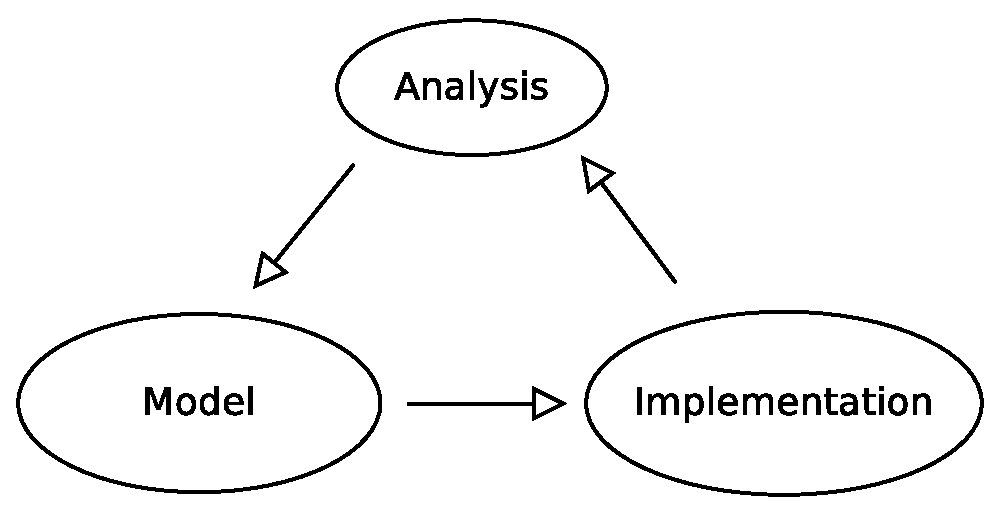
\includegraphics[height=6in]{methodology}}
        \else
        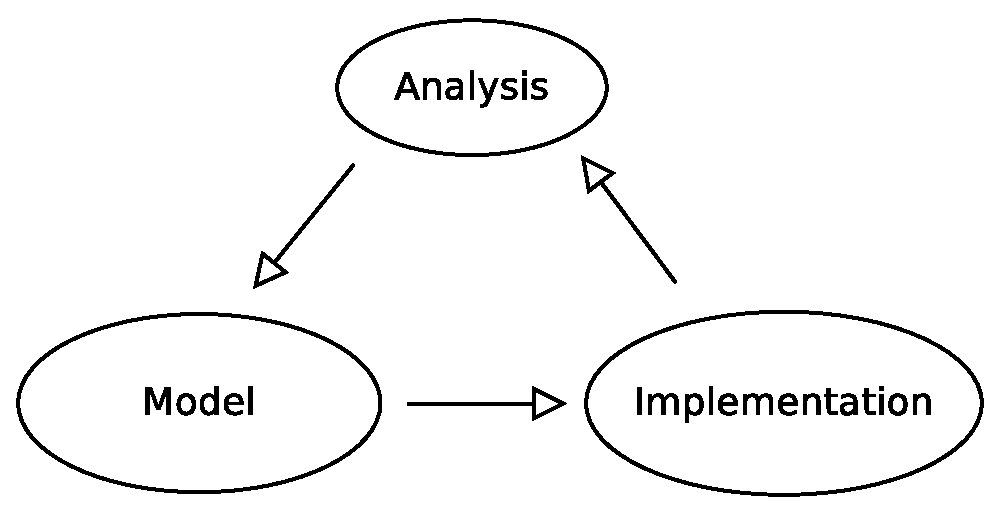
\includegraphics[bb = 92 86 545 742, height=6in]{methodology}
        \fi
        \caption{Instructional Simulate model for this study}
    \end{center}
\end{figure}

In the stage \verb|Model| and \verb|Implementation|, Use \verb|OPNET| as main tool. Because of \verb|OPNET| have provide a basic platform before progressing to the \verb|OBS| model. \verb|OPNET| simulation model library provide a series of simulation model for customer. On the basis of these simulation model, we can customize our network model and run a simulation. \verb|OPNET| simulation model library separate with the network simulation engine(\verb|OPNET|
Modeler,\verb|ITGuru|,Application DecisionGuru). This architecture is very convenient for model change and upgrade. For this study, we can deploy our congestion control algorithm to a \verb|OBS| network which build with \verb|OPNET| easily. 

To generate burst from all ingress node, we need to assume the arrive process follow certain distribution. That may be some common randomness processes. Such as negative exponential distribution, geometric distribution, drop-tail distribution. Thus we need to know how to generate this randomness process meet some distribution requirement. 

In order to measure our congestion control mechanism achievements. We need to setup a optimal target. In this study, that is maximum throughput and minimum burst loss and block ratio. It is hard to work out through pure analysis method. So we need to collect data from simulation. We can do some comparative experiments. Such as compare the throughput of two case. One with congestion control, the other without congestion control. Also, 
use some generally knowledge truth in queuing theory and probability theory to let us get closed optimal target step by step. It is a very good idea to make our data intuitive with data visualization technology.

\newpage
\section{About congestion control}
To understand what is congestion control. The first question what causes congestion must be answer. Fortunately, the answer is simple, congestion occurs when the total traffic load is greater than network bottleneck capacity. Especially, OBS take one-way reservation to avoid the long end-to-end setup times and without buffer on intermediate router. Once contention occurs, some or all of data burst have to be dropped. Hence, contention is inherent to the OBS technique and
contention issue could affect tremendously the network performance in terms of burst blocked rate and throughput.

General speaking, the contention problem is due to the lack of communication between the nodes and the absence of global coordination between the edge routers and core routers. Congestion issue will lead to a large waste of resource due to drop of bursts on last one router before destination since fail to compete fail. Even worse, the network is statistical multiplexing, many burst may share a link, that lead to load is not balance over all core routers. Some core router may
overload, the others may be idle.  

There are two approaches to handle burst contention problem: bursts contention resolution and burst congestion control. The burst contention resolution approaches should have capacity to store burst with fiber delay lines (FDLs) \cite{fdl}, deflection routing \cite{deflection}, and wavelength conversion \cite{wavelenghtconv}. These approaches can reduce burst loss rate by absorbing short-term burst congestion. But if the burst congestion lasts long, all of above
approaches can't reduce burst loss rate anymore. Even worse, they may introduce longer end-to-end delay and enhance congestion impact. 

The burst congestion control mechanism handle the burst congestion by controlling the data burst transmission rate at the optical network edge. There are two paradigm to limit the source flow rate, refer as open-loop and closed-loop congestion control. The main different between these two mechanism is that closed-loop is dynamic adaptive system with feedback message. Open-loop is a per-define system without dynamic adjust stage.  There are two jointly operating mechanisms, namely a
burst congestion detection and a burst control algorithm in closed-loop network\cite{longterm}. Thus, in the feedback-based network it is required for the core router to work out 3W1H (what,where,when,how) question. What information should feedback to network edge router? Which router should monitor the network information and report to edge router? When this statistic result can detect the congestion and tell the edge router to reduce transmission
rate? On the other side the core router should tell when the edge router increase transmission rate to keep network throughput high? The last question is how to detect and predict the network congestion? How to guarantee fairness and self-organizing? 

%However, there are some misunderstandings about the causes and solutions of congestion control.
%
%\begin{enumerate}
%    \item Congestion is caused by the shortage of buffer space. The problem will be solved when the cost of memory becomes cheap enough to allow very large memory. Larger buffers are useful only for very short term congestions and will cause undesirable long delays. The long queue and long delay introduced by large memory is undesirable for many applications.
%
%    \item Congestion is caused by slow links. The problem will be solved when high-speed links become available. It is not always the case; sometimes increases in link bandwidth can aggravate the congestion problem because higher speed links may make the network more unbalanced. If two sources begin to send to destination 1 at their peak rate, congestion will occur at the switch. Higher speed links can make the congestion condition in the switch even worse.
%
%    \item Congestion is caused by slow processors. The problem will be solved when processor speed is improved. This statement can be explained to be wrong similarly to the second one. Faster processors will transmit more data per unit time. If several nodes begin to transmit to one destination simultaneously at their peak rate, the target will soon be overwhelmed. Congestion is a dynamic problem, and any static solutions are therefore not sufficient to solve the problem.
%        All the issues presented above: buffer shortage, slow link, slow processor are symptoms, not the causes of congestion. Proper congestion management mechanisms are more important than ever.
%\end{enumerate}

\cleardoublepage
\section{Motivation}

\begin{figure}[!htbp]
    \label{fig:ideal_congestion_control}
    \begin{center}
        \leavevmode
        \ifpdf
        \resizebox{90mm}{!}{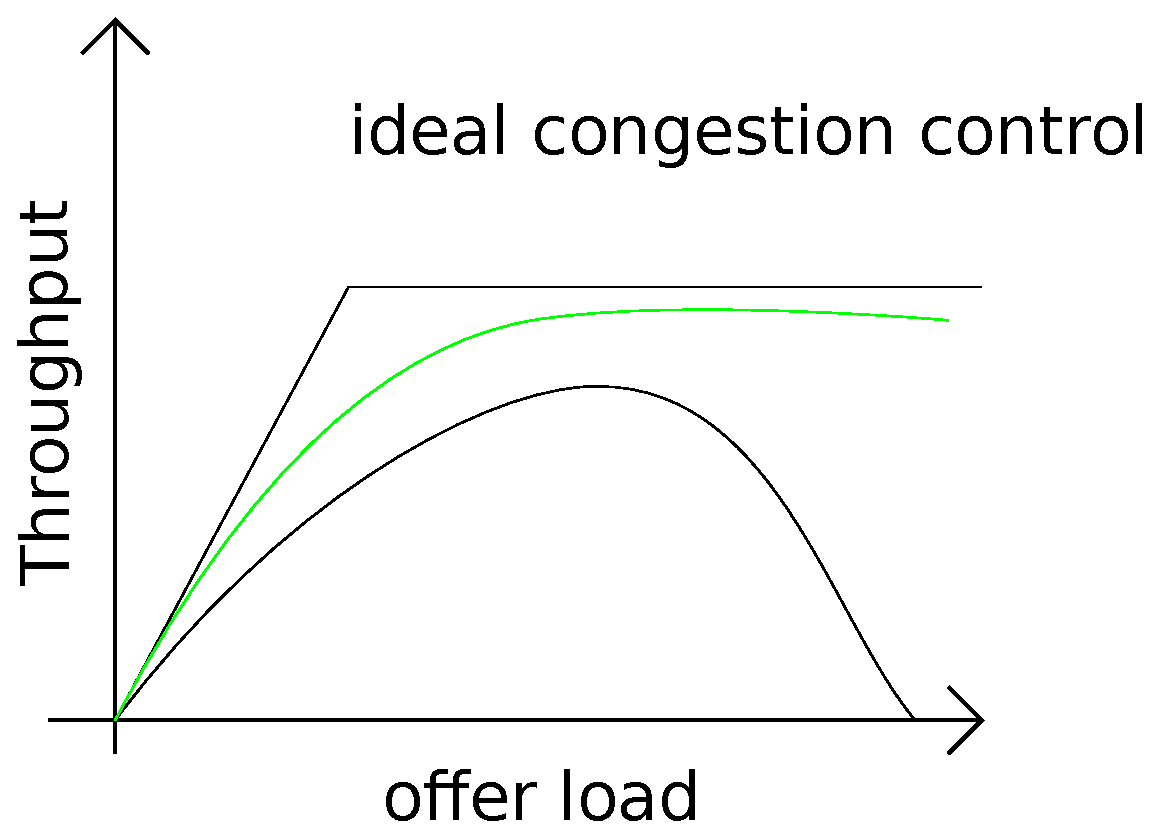
\includegraphics[height=6in]{ideal_congestion_control}}
        \else
        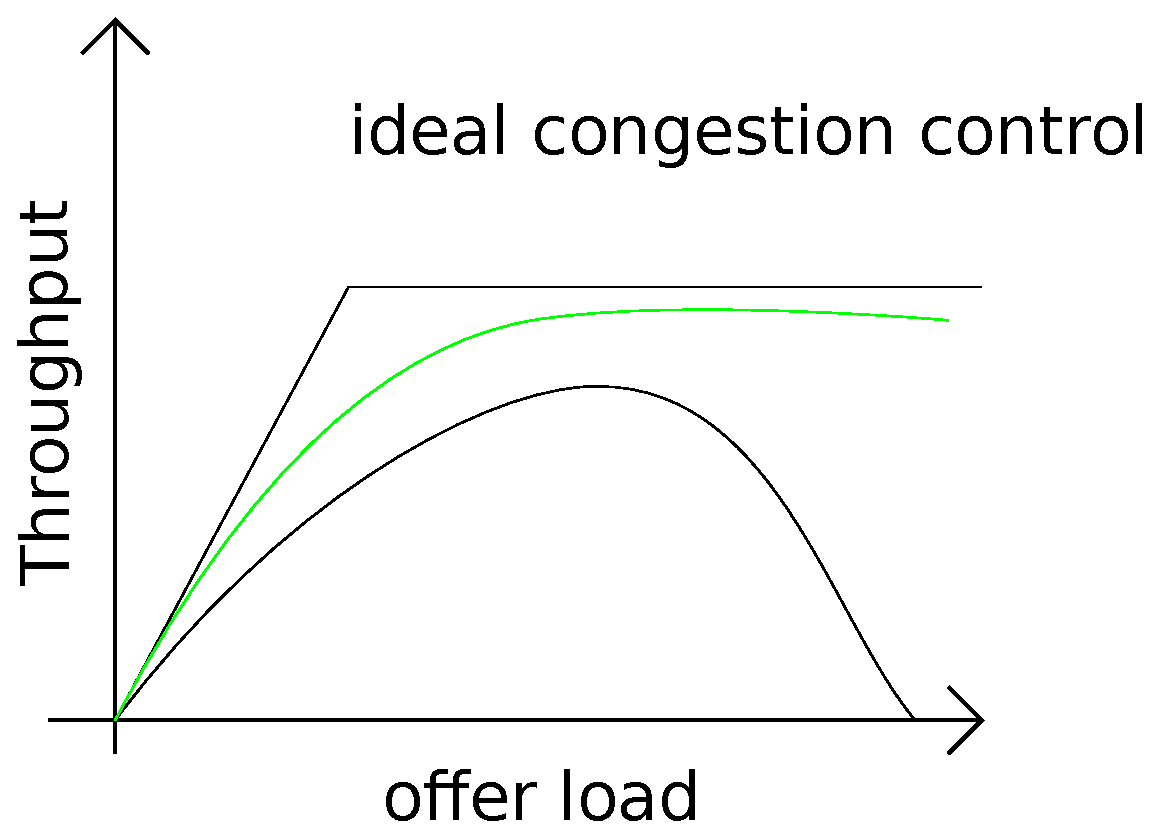
\includegraphics[bb = 92 86 545 742, height=6in]{ideal_congestion_control}
        \fi
        \caption{Congestion Control}
    \end{center}
\end{figure}

As figure \ref{fig:ideal_congestion_control} shows, The performance of network would reduce to zero if without any control. The ideal congestion control will enhance the network stability, and gain the capacity of network. However, in real network, the reaction delay much be token account. It only be closed to the ideal line. The green line show the real world congestion control. It may jitter since control packet loss or expired. In this study, I will develop a congestion control to
improve the throughput of network and reduce burst blocked probability.

There are several goals that congestion mechanism should achieve, the cost of implementation and deploy is cheap. That is said minimize additional hardware requirement and limited by router ability. Be fair among to all user.   

Congestion control is a comprehensive problem. The effective is very limited by control with any single method. Monitor and rate controller should co-operate to expand the effective. It may work with other mechanism, something like early drop packet, soft contention strategy.  

\section{Related Work}
As a new switching technology which has not been standardized yet, OBS faces many problems and challenges. However, there are also many researchers and new achievements. In resolving the issues of contention and the associated loss bursts issue. There are some other related studies. 

The most important and related study is contention resolution. As mention above, there are three ways to resolve burst contention. Fiber delay line, wavelength conversion and deflection routing by now. They are for a same goal. When contention occurs, they can buffer it instead of drop it. But these three method are not viable now. They all have their own shortcomings. Optical buffering currently can only be implemented using FDL. But this type of optical buffer is
usually small and it does not scale up. The wavelength may have some potential since the number of wavelengths that can be coupled together onto a single fiber continues to increase. In view of deflected routing, the end-to-end delay for an optical burst may be unacceptably high. But fortunately research on these contention resolution are going on. Once the breakthrough of these problems will also provide help for congestion control. 

Nowadays, IP packet switching already dominates global communications. But it cannot keep up with the Internet traffic demand. Many researchers are studying a new scheme to replace it. In electronic domain, ATM network has matured and is not far from being feasible. Other researcher have proposed integrate circuit switching in the core and packet switching in the edges as next generation network architecture. All of these efforts are aimed at accommodating for the traffic growth in the Internet. Study on the OBS can draw on
their achievements. Also include conventional TCP congestion control. 



%%% Local Variables: 
%%% mode: latex
%%% TeX-master: "../thesis"
%%% End: 

%\include{Chapter2/chapter2}
%\include{Chapter3/chapter3}
%\def\baselinestretch{1}
\chapter{Conclusions}
\ifpdf
    \graphicspath{{Conclusions/ConclusionsFigs/PNG/}{Conclusions/ConclusionsFigs/PDF/}{Conclusions/ConclusionsFigs/}}
\else
    \graphicspath{{Conclusions/ConclusionsFigs/EPS/}{Conclusions/ConclusionsFigs/}}
\fi

%\def\baselinestretch{1.66}

Up to now, we have know that DWDM take the bottleneck of networks from bandwidth to switching technology. OBS emerge as this requirement. OBS have many advantage with the advance of DWDM technology. It have great potential to be next generation switching technology in the core network. Since it have some special feature. Such as not require buffer, separation of transmission and control packet. 

As mention above chapter, contention is very possible occurs in ideal network without congestion control. OBS have no standardize yet. Many researcher work on this challenging topic. The main research method is simulation. Overview of all previous, they have build a theory framework to solve congestion collapse for OBS. That is three steps: detect, feedback, reaction. They are different in implementation detail. All mechanism are tightly coupled with the burst assembly mechanism at the
ingress edge router. This was decided by two reasons. The First is all intelligence resides in the edge router, which are at the same time the buffer and the processor. The second is the hurdle for congestion is lacking of communication between the nodes and the absence of global coordination between the edge routers and core routers. Hence, monitor on corn router and controller on edge router will be focus on the future work. 



%%% ----------------------------------------------------------------------

% ------------------------------------------------------------------------

%%% Local Variables: 
%%% mode: latex
%%% TeX-master: "../thesis"
%%% End: 


\backmatter % book mode only
%\appendix
%\include{Appendix1/appendix1}
%\include{Appendix2/appendix2}


%new
%\bibliographystyle{plainnat}
%endnew
\pagestyle{plain}
\bibliographystyle{Classes/CUEDbiblio}
%\bibliographystyle{Classes/jmb}
%\bibliographystyle{plainnat} %this works with package natbib
%\bibliographystyle{Classes/jmb} % bibliography style
\renewcommand{\bibname}{References} % changes default name Bibliography to References
\bibliography{References/references} % References file

\end{document}
